\iffalse
\let\negmedspace\undefined
\let\negthickspace\undefined
\documentclass[journal,12pt,twocolumn]{IEEEtran}
\usepackage{cite}
\usepackage{amsmath,amssymb,amsfonts,amsthm}
\usepackage{algorithmic}
\usepackage{graphicx}
\usepackage{textcomp}
\usepackage{xcolor}
\usepackage{txfonts}
\usepackage{listings}
\usepackage{enumitem}
\usepackage{mathtools}
\usepackage{gensymb}
\usepackage{comment}
\usepackage[breaklinks=true]{hyperref}
\usepackage{tkz-euclide} 
\usepackage{listings}
\usepackage{gvv}  
\usepackage{tikz}
\usepackage{circuitikz} 
\usepackage{caption}

\def\inputGnumericTable{}                                
\usepackage[latin1]{inputenc}                 
\usepackage{color}                            
\usepackage{array}                            
\usepackage{longtable}                        
\usepackage{calc}                            
\usepackage{multirow}                      
\usepackage{hhline}                           
\usepackage{ifthen}                          
\usepackage{lscape}
\usepackage{amsmath}
\newtheorem{theorem}{Theorem}[section]
\newtheorem{problem}{Problem}
\newtheorem{proposition}{Proposition}[section]
\newtheorem{lemma}{Lemma}[section]
\newtheorem{corollary}[theorem]{Corollary}
\newtheorem{example}{Example}[section]
\newtheorem{definition}[problem]{Definition}
\newcommand{\BEQA}{\begin{eqnarray}}
\newcommand{\EEQA}{\end{eqnarray}}
\newcommand{\define}{\stackrel{\triangle}{=}}
\theoremstyle{remark}
\newtheorem{rem}{Remark}

\begin{document}
\title{}
\author{Sasa Mardi, EE23BTECH11222}
\date{}
\maketitle
\textbf{Question 10.5.2-9:}
If the 3rd and the 9th terms of an AP are 4 and -8, respectively, which term of this AP is zero? \\
\solution
\fi
\begin{table}[h!]
    \centering
    \caption{Input Parameters}
    \label{tab:10.5.2.9.1}
    \begin{tabular}{ | c | c | c | }
        \hline
        Parameter & Value & Description \\
        \hline
        $x(n)$ & $x(0) + (n)d$ & ${(n+1)}^{th}$ term of the AP \\
        \hline
        $x(0) + 2d$ & 4 & Third term of the AP \\
        \hline
        $x(0) + 8d$ & -8 & Ninth term of the AP \\
        \hline
        $x(0)$ & - & First term of the AP \\
        \hline
        $d$ & - & Common difference of the AP \\
        \hline
    \end{tabular}
\end{table}

\begin{equation}
\left(
\begin{array}{r}
x(0) \\
8d \\
-8 
\end{array}
\right)
-
\left(
\begin{array}{r}
x(0) \\
2d \\
4
\end{array}
\right)
=
\left(
\begin{array}{r}
0 \\
6d \\
-12
\end{array}
\right)
\end{equation}
\begin{align}
6d &= -12 \\
\implies d &= -2 
\end{align}
Substitute d = -2 into:
\begin{align}
x(0) &= 4 - 2d\\
&= 4 - 2(-2)\\
&= 8
\end{align}
Substitute x(0) = 8 and d = -2 into:
\begin{align}
x(n) = x(0) + (n)d &= 0 \\
8 + (n)(-2) &= 0 \\
n &= 4
\end{align}
Term number = n + 1 = 5 \\
The term where the value is zero in the given arithmetic progression is the 5th term.\\
\begin{enumerate}
\item Finding $x(n)$ \\
The series is an arithmetic progression.
\begin{align}
x(n) = (x(0) + n(-2))(u(n))
\end{align}
\begin{figure}[h!]
    \centering
    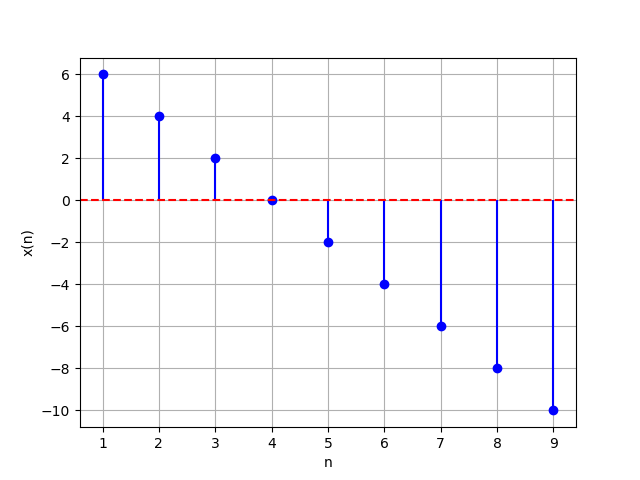
\includegraphics[width=\columnwidth]{ncert-maths/10/5/2/9/figs/xn.png}
    \caption{Plot of $x(n)$ vs $n$}
    \label{fig:10.5.2.9.1}
\end{figure}
\item Z-transform of $x(n)$ \\
\begin{align}
\frac{x(0)}{1 - z^{-1}} + \frac{dz^{-1}}{(1 - z^{-1})^2} \quad \forall \quad |z| > 1
\end{align}
Using the values from \tabref{tab:10.5.2.9.1}:
\begin{align}
\frac{8}{1 - z^{-1}} + \frac{-2z^{-1}}{(1 - z^{-1})^2} \quad \forall \quad |z| > 1
\end{align}
\end{enumerate}


